%% IJCAS submission, FULL-LENGTH version: main.tex plus every figure and table of the supplement.
%% Built with the official IJCAS.cls (template of 19 Feb 2026).
%% Every number in the text is a macro generated by paper/scripts/make_tables_v2.py
%% (tables/numbers.tex); tables are generated by the same script. Do not type numbers by hand.
\documentclass{IJCAS}

\usepackage{url}
\usepackage{array,tabularx}
\usepackage{multicol}
\usepackage{algorithm}
\usepackage{algorithmic}
\usepackage{multirow}
\usepackage{graphicx}

\journalvolumn{VV}
\journalnumber{X}
\journalyear{YYYY}
\setarticlestartpagenumber{1}

\allowdisplaybreaks
\newcommand{\VfrozenKL}{was exactly zero}
\newcommand{\VextMeanLo}{0.79}
\newcommand{\VextMeanHi}{1.24}
\newcommand{\VextMax}{6.53}
\newcommand{\VfixL}{0.125}
\newcommand{\VfixG}{0.9}
\newcommand{\VfixLm}{0.125}
\newcommand{\VfixGm}{1.0}
\newcommand{\VadA}{0.05}
\newcommand{\VadB}{0.025}
\newcommand{\VadAm}{0.05}
\newcommand{\VadBm}{0.05}
\newcommand{\VbppL}{0.125}
\newcommand{\VbppG}{1.2}
\newcommand{\VtuneRa}{0.37}
\newcommand{\VtuneRb}{0.24}
\newcommand{\VtuneRc}{0.26}
\newcommand{\VrlppLmin}{0.05}
\newcommand{\VrlppLmax}{0.86}
\newcommand{\VrlppGmin}{0.87}
\newcommand{\VrlppGmax}{1.26}
\newcommand{\VrlppGstd}{0.09}
\newcommand{\VrLk}{$-$0.68}
\newcommand{\VrGk}{0.70}
\newcommand{\VrlppLmed}{0.44}
\newcommand{\VrlppLlo}{0.05}
\newcommand{\VrlppLhi}{0.90}
\newcommand{\VrlppLband}{57}
\newcommand{\VtExpert}{42.5}
\newcommand{\VtFix}{18.5}
\newcommand{\VtFixM}{42.2}
\newcommand{\VtBpp}{42.5}
\newcommand{\VcompPPO}{98}
\newcommand{\VcompPPOacc}{74}
\newcommand{\VgPPO}{89.8}
\newcommand{\VgPPOacc}{83.1}
\newcommand{\VnEpisodes}{8400}
\newcommand{\VrmseExpert}{1.07}
\newcommand{\VrmseDagger}{1.06}
\newcommand{\VrmseDP}{1.77}
\newcommand{\VrmseDPacc}{2.14}
\newcommand{\VrmsePPO}{5.12}
\newcommand{\VrmsePPOacc}{6.49}
\newcommand{\VrmseBpp}{0.28}
\newcommand{\VrmseFix}{0.34}
\newcommand{\VrmseAd}{0.42}
\newcommand{\VrmseRL}{1.83}
\newcommand{\VrmseRLld}{1.57}
\newcommand{\VrmsePubBead}{4.38}
\newcommand{\VrmsePubRL}{3.68}
\newcommand{\VrmseFixOrig}{3.85}
\newcommand{\VrmseAdOrig}{10.12}
\newcommand{\VrmseFixM}{0.31}
\newcommand{\VrmseAdM}{0.35}
\newcommand{\VrmseRLM}{2.40}
\newcommand{\VrewExpert}{715}
\newcommand{\VrewDagger}{715}
\newcommand{\VrewDP}{694}
\newcommand{\VrewPPO}{534}
\newcommand{\VexRewBzero}{746}
\newcommand{\VexRewBnoise}{764}
\newcommand{\VexRewPzero}{836}
\newcommand{\VexRewPnoise}{725}
\newcommand{\VexRmseZero}{0.91}
\newcommand{\VexRmseNoise}{2.92}
\newcommand{\VexTZero}{48}
\newcommand{\VexTNoise}{61}
\newcommand{\VexStd}{0.61}
\newcommand{\VdiagDPDagDetrew}{747}
\newcommand{\VdiagDPDagDetrmse}{0.86}
\newcommand{\VdiagDPDagStorew}{749}
\newcommand{\VdiagDPDagStormse}{1.05}
\newcommand{\VdiagDPFtDetrew}{729}
\newcommand{\VdiagDPFtDetrmse}{1.56}
\newcommand{\VdiagDPFtStorew}{729}
\newcommand{\VdiagDPFtStormse}{1.69}
\newcommand{\VdiagDPStdEnd}{0.13}
\newcommand{\VdiagDPaccDagDetrew}{838}
\newcommand{\VdiagDPaccDagDetrmse}{0.86}
\newcommand{\VdiagDPaccDagStorew}{829}
\newcommand{\VdiagDPaccDagStormse}{1.05}
\newcommand{\VdiagDPaccFtDetrew}{811}
\newcommand{\VdiagDPaccFtDetrmse}{1.84}
\newcommand{\VdiagDPaccFtStorew}{804}
\newcommand{\VdiagDPaccFtStormse}{1.92}
\newcommand{\VdiagDPaccStdEnd}{0.12}
\newcommand{\VklLo}{0.010}
\newcommand{\VklHi}{0.031}
\newcommand{\VevLo}{0.86}
\newcommand{\VevHi}{0.98}
\newcommand{\VnRefs}{493}
\newcommand{\VnInst}{60}
\newcommand{\VnSynthEval}{100}
\newcommand{\VnRerun}{22}
\newcommand{\VekSelC}{1}
\newcommand{\VekRmseC}{1.07}
\newcommand{\VekFailC}{4}
\newcommand{\VekRmseThreeC}{3.59}
\newcommand{\VekSelN}{2}
\newcommand{\VekRmseN}{1.15}
\newcommand{\VekFailN}{4}
\newcommand{\VekRmseThreeN}{2.39}
\newcommand{\VselSame}{32}
\newcommand{\VselTotal}{45}
\newcommand{\VselMaxDiff}{0.48}
\newcommand{\VselMedDiff}{0.04}
\newcommand{\VadRmseSel}{0.510}
\newcommand{\VadRmseConst}{0.509}
\newcommand{\VpilotPmrmse}{6.69}
\newcommand{\VpilotPmscore}{0.750}
\newcommand{\VpilotPhrmse}{7.12}
\newcommand{\VpilotPhscore}{0.851}
\newcommand{\VpilotPzrmse}{7.82}
\newcommand{\VpilotPzscore}{0.811}
\newcommand{\VlatAccP}{29.3}
\newcommand{\VlatAccFrac}{12.4}
\newcommand{\VlatAccMaxM}{9.4}
\newcommand{\VscaleLo}{4.3}
\newcommand{\VscaleMed}{6.5}
\newcommand{\VscaleHi}{9.8}
\newcommand{\VcmpPoneDiff}{0.75}
\newcommand{\VcmpPoneLo}{0.62}
\newcommand{\VcmpPoneHi}{0.87}
\newcommand{\VcmpPoneBetter}{0}
\newcommand{\VcmpPoneP}{0.0078}
\newcommand{\VcmpPfourDiff}{$-$0.79}
\newcommand{\VcmpPfourLo}{$-$0.92}
\newcommand{\VcmpPfourHi}{$-$0.64}
\newcommand{\VcmpPfourBetter}{8}
\newcommand{\VcmpPfourP}{0.0078}
\newcommand{\VcmpRLJLDiff}{0.26}
\newcommand{\VcmpRLJLLo}{$-$0.30}
\newcommand{\VcmpRLJLHi}{0.87}
\newcommand{\VcmpRLJLBetter}{1}
\newcommand{\VcmpRLJLP}{0.0234}
\newcommand{\VcmpBppDagDiff}{$-$0.64}
\newcommand{\VcmpBppDagLo}{$-$0.77}
\newcommand{\VcmpBppDagHi}{$-$0.48}
\newcommand{\VcmpBppDagBetter}{8}
\newcommand{\VcmpBppDagP}{0.0078}
\newcommand{\VcmpBppTeachDiff}{0.15}
\newcommand{\VcmpBppTeachLo}{0.11}
\newcommand{\VcmpBppTeachHi}{0.18}
\newcommand{\VcmpBppTeachBetter}{0}
\newcommand{\VcmpBppTeachP}{0.0078}
\newcommand{\VrmseDaggerBpp}{0.42}
\newcommand{\VbcValLow}{2.18}
\newcommand{\VbcValOne}{1.57}
\newcommand{\VbcValHigh}{1.09}
\newcommand{\VbcValDagger}{0.86}
\newcommand{\VbcSel}{10}
\newcommand{\VrmseDPbcHigh}{1.26}
\newcommand{\VcmpBcDagDiff}{0.20}
\newcommand{\VcmpBcDagLo}{0.15}
\newcommand{\VcmpBcDagHi}{0.26}
\newcommand{\VcmpBcDagBetter}{0}
\newcommand{\VcmpBcDagP}{0.0078}
\newcommand{\VcmpBcDPDiff}{$-$0.50}
\newcommand{\VcmpBcDPLo}{$-$0.75}
\newcommand{\VcmpBcDPHi}{$-$0.31}
\newcommand{\VcmpBcDPBetter}{8}
\newcommand{\VcmpBcDPP}{0.0078}
\newcommand{\VrmseTrueExpert}{1.60}
\newcommand{\VrmseTrueBpp}{1.24}
\newcommand{\VrmseTrueDagger}{1.60}
\newcommand{\VrmseTrueFix}{1.25}
\newcommand{\VrmseTrueFixM}{1.23}
\newcommand{\VrmseTrueDP}{2.26}
\newcommand{\VrmseTrueRL}{2.22}
\newcommand{\VrmseTrueDaggerBpp}{1.24}
\newcommand{\VtruePoneDiff}{0.36}
\newcommand{\VtruePoneLo}{0.22}
\newcommand{\VtruePoneHi}{0.51}
\newcommand{\VtruePoneBetter}{0}
\newcommand{\VtruePoneP}{0.0078}
\newcommand{\VtruePfourDiff}{$-$0.36}
\newcommand{\VtruePfourLo}{$-$0.49}
\newcommand{\VtruePfourHi}{$-$0.23}
\newcommand{\VtruePfourBetter}{8}
\newcommand{\VtruePfourP}{0.0078}
\newcommand{\VtrueBppDagDiff}{$-$0.36}
\newcommand{\VtrueBppDagLo}{$-$0.52}
\newcommand{\VtrueBppDagHi}{$-$0.19}
\newcommand{\VtrueBppDagBetter}{7}
\newcommand{\VtrueBppDagP}{0.0156}
\newcommand{\VtrueBppTeachDiff}{0.00}
\newcommand{\VtrueBppTeachLo}{$-$0.03}
\newcommand{\VtrueBppTeachHi}{0.04}
\newcommand{\VtrueBppTeachBetter}{3}
\newcommand{\VtrueBppTeachP}{0.8438}
\newcommand{\VtrueBppFixMDiff}{0.01}
\newcommand{\VtrueBppFixMLo}{$-$0.03}
\newcommand{\VtrueBppFixMHi}{0.05}
\newcommand{\VtrueBppFixMBetter}{2}
\newcommand{\VtrueBppFixMP}{0.4609}
\newcommand{\VcmpBppFixMDiff}{0.12}
\newcommand{\VcmpBppFixMLo}{0.08}
\newcommand{\VcmpBppFixMHi}{0.15}
\newcommand{\VcmpBppFixMBetter}{0}
\newcommand{\VcmpBppFixMP}{0.0078}
\newcommand{\VrankCorr}{0.993}
\newcommand{\VnPrimTrue}{4}
\newcommand{\VspMin}{11.1}
\newcommand{\VspMax}{23.5}
\newcommand{\VspMed}{16.6}
\newcommand{\VspTestMin}{11.1}
\newcommand{\VspTestMax}{21.5}
\newcommand{\VthreePubBeadLo}{2.45}
\newcommand{\VthreePubBeadHi}{4.05}
\newcommand{\VthreeFixOrigLo}{3.62}
\newcommand{\VthreeFixOrigHi}{5.54}
\newcommand{\VthreePubRLLo}{3.72}
\newcommand{\VthreePubRLHi}{4.58}
\newcommand{\VthreeFixLo}{0.27}
\newcommand{\VthreeFixHi}{0.50}
\newcommand{\VthreeExpertLo}{0.94}
\newcommand{\VthreeExpertHi}{1.36}
\newcommand{\VrestPubBead}{5.02}
\newcommand{\VthreePubBeadMean}{3.32}
\newcommand{\VwithinExpert}{96.9}
\newcommand{\VwithinBpp}{99.8}
\newcommand{\VwithinDagger}{97.5}
\newcommand{\VwithinDP}{92.7}
\newcommand{\VwithinPPO}{60.4}
\newcommand{\VwithinRL}{96.0}
\newcommand{\VwithinFix}{99.8}
\newcommand{\VwithinAd}{99.6}
\newcommand{\VstK}{512}
\newcommand{\VstKs}{0.01}
\newcommand{\VstKm}{1024}
\newcommand{\VstKsm}{1}
\newcommand{\VstNgrid}{220}
\newcommand{\VrmseSt}{4.12}
\newcommand{\VcompSt}{88}
\newcommand{\VrmseTrueSt}{4.44}
\newcommand{\VrmseStM}{3.56}
\newcommand{\VcompStM}{88}
\newcommand{\VrmseTrueStM}{3.90}
\newcommand{\VcmpStFixDiff}{3.78}
\newcommand{\VcmpStFixLo}{3.45}
\newcommand{\VcmpStFixHi}{4.05}
\newcommand{\VcmpStFixBetter}{0}
\newcommand{\VcmpStFixP}{0.0078}
\newcommand{\VcmpStFixMDiff}{3.25}
\newcommand{\VcmpStFixMLo}{2.88}
\newcommand{\VcmpStFixMHi}{3.54}
\newcommand{\VcmpStFixMBetter}{0}
\newcommand{\VcmpStFixMP}{0.0078}
\newcommand{\VtrueStFixDiff}{3.19}
\newcommand{\VtrueStFixLo}{2.88}
\newcommand{\VtrueStFixHi}{3.44}
\newcommand{\VtrueStFixBetter}{0}
\newcommand{\VtrueStFixP}{0.0078}
\newcommand{\VtrueStFixMDiff}{2.67}
\newcommand{\VtrueStFixMLo}{2.31}
\newcommand{\VtrueStFixMHi}{2.97}
\newcommand{\VtrueStFixMBetter}{0}
\newcommand{\VtrueStFixMP}{0.0078}
\newcommand{\VfrontStM}{2.22}
\newcommand{\VrearStM}{3.56}
\newcommand{\VfrontFixM}{4.83}
\newcommand{\VrearFixM}{0.31}
\newcommand{\VrmseDtFix}{3.95}
\newcommand{\VcompDtFix}{88}
\newcommand{\VrmseDtRL}{5.68}
\newcommand{\VcompDtRL}{73}
\newcommand{\VrmseDtRLLo}{3.29}
\newcommand{\VrmseDtRLHi}{7.24}
\newcommand{\VrmseDrFix}{34.84}
\newcommand{\VcompDrFix}{0}
\newcommand{\VrmseDrRL}{23.52}
\newcommand{\VcompDrRL}{2}
\newcommand{\VrmseDrRLLo}{13.29}
\newcommand{\VrmseDrRLHi}{29.66}
\newcommand{\VdynTRLFixDiff}{1.73}
\newcommand{\VdynTRLFixLo}{$-$0.02}
\newcommand{\VdynTRLFixHi}{3.38}
\newcommand{\VdynTRLFixBetter}{2}
\newcommand{\VdynTRLFixP}{0.0547}
\newcommand{\VdynRRLFixDiff}{$-$11.32}
\newcommand{\VdynRRLFixLo}{$-$17.53}
\newcommand{\VdynRRLFixHi}{$-$4.71}
\newcommand{\VdynRRLFixBetter}{8}
\newcommand{\VdynRRLFixP}{0.0078}
\newcommand{\VrmseDtFixR}{1.91}
\newcommand{\VtrueRmseDtFixR}{2.30}
\newcommand{\VcompDtFixR}{100}
\newcommand{\VrmseDtFixH}{1.83}
\newcommand{\VtrueRmseDtFixH}{2.31}
\newcommand{\VcompDtFixH}{100}
\newcommand{\VrmseDtStR}{2.66}
\newcommand{\VtrueRmseDtStR}{3.11}
\newcommand{\VcompDtStR}{100}
\newcommand{\VrmseDtRLR}{5.26}
\newcommand{\VtrueRmseDtRLR}{5.38}
\newcommand{\VcompDtRLR}{82}
\newcommand{\VdynDtFixStDiff}{$-$0.75}
\newcommand{\VdynDtFixStLo}{$-$1.29}
\newcommand{\VdynDtFixStHi}{$-$0.18}
\newcommand{\VdynDtFixStBetter}{6}
\newcommand{\VdynDtFixStP}{0.0781}
\newcommand{\VdynDtFixRLDiff}{$-$3.35}
\newcommand{\VdynDtFixRLLo}{$-$4.91}
\newcommand{\VdynDtFixRLHi}{$-$2.10}
\newcommand{\VdynDtFixRLBetter}{8}
\newcommand{\VdynDtFixRLP}{0.0078}
\newcommand{\VrmseDrFixR}{3.23}
\newcommand{\VtrueRmseDrFixR}{3.59}
\newcommand{\VcompDrFixR}{88}
\newcommand{\VrmseDrFixH}{3.09}
\newcommand{\VtrueRmseDrFixH}{3.53}
\newcommand{\VcompDrFixH}{100}
\newcommand{\VrmseDrStR}{3.58}
\newcommand{\VtrueRmseDrStR}{3.83}
\newcommand{\VcompDrStR}{88}
\newcommand{\VrmseDrRLR}{6.73}
\newcommand{\VtrueRmseDrRLR}{6.82}
\newcommand{\VcompDrRLR}{50}
\newcommand{\VdynDrFixStDiff}{$-$0.36}
\newcommand{\VdynDrFixStLo}{$-$0.90}
\newcommand{\VdynDrFixStHi}{0.32}
\newcommand{\VdynDrFixStBetter}{7}
\newcommand{\VdynDrFixStP}{0.1953}
\newcommand{\VdynDrFixRLDiff}{$-$3.50}
\newcommand{\VdynDrFixRLLo}{$-$5.67}
\newcommand{\VdynDrFixRLHi}{$-$1.94}
\newcommand{\VdynDrFixRLBetter}{8}
\newcommand{\VdynDrFixRLP}{0.0078}
\newcommand{\VbppGainHighDr}{1.60}

\graphicspath{{figures/}}
\makeatletter\let\tabinput\@@input\makeatother % expandable input for table bodies

\begin{document}

\title{Learned Direct Actuation versus Tuned and RL-Tuned Pure Pursuit: A Controlled Comparison for Path Tracking}

\author{Dileep Banothu and N. Sanjay Varma*}

\begin{abstract}
Two parameters govern Pure Pursuit (PP) tracking, its steering gain and its lookahead distance, and reinforcement learning (RL) has recently been integrated with PP by letting an agent tune both online. We compare such integration of learning with classical control against learning that replaces the geometric law. A network drives a ``bead'' (a point mass) by choosing its acceleration along references extracted from images and is trained by imitation (DAgger), Proximal Policy Optimization (PPO), or both. It is compared with tuned PP, an adaptation of RL-tuned PP, and the PP law run on the bead, under one simulator and lap rule, on eight held-out F1TENTH circuits with five training seeds. Imitating a hand-written rule, the bead matches that rule (\VrmseDagger~cm RMSE). With our PPO budget and settings, PPO did not improve this imitation policy. Tuned PP reaches \VrmseFixM~cm at the bead's speed, and \VrmseBpp~cm when run on the bead, so the gap stems from the control law, not the vehicle; against the true centerlines it shrinks from \VcmpPoneDiff\ to \VtruePoneDiff~cm but keeps its sign. Imitating the PP law instead, the network reaches \VrmseDaggerBpp~cm and matches tuned PP against the true centerlines. On a dynamic single-track car, gains must be re-tuned; PP then stays the most accurate car controller (\VrmseDtFixR~cm), with an unclear lead over Stanley. A naive protocol with test leakage and untuned baselines would have reversed these conclusions.
\end{abstract}

\begin{keywords}
F1TENTH, imitation learning, path tracking, pure pursuit, reinforcement learning.
\end{keywords}

\maketitle

\makeAuthorInformation{
Dileep Banothu and N. Sanjay Varma are with the Indian Institute of Information Technology Sri City, Sri City, Andhra Pradesh 517646, India (e-mails: [D. Banothu e-mail], sanjayvarma.n24@iiits.in).\\
* Corresponding author.
}

\runningtitle{YYYY}{Dileep Banothu and N. Sanjay Varma}{Learned Direct Actuation versus Tuned and RL-Tuned Pure Pursuit}{xxx}{xxxx}{x}


\section{Introduction}
Between the planner and the actuators of an autonomous vehicle sits a path tracker, which converts the planned path into motion commands. On small-scale racing cars such as F1TENTH~\cite{okelly2020} the tracker is typically geometric, and Pure Pursuit (PP)~\cite{coulter1992,snider2009} is the most common choice: it aims at the path point lying a lookahead distance $L_d$ ahead and scales the resulting steering by a gain $g$. The choice of $L_d$ is a compromise---a small value responds fast but oscillates, a large value is smooth but cuts corners.

Computational intelligence can be integrated with such a controller in two ways. In RL-tuned PP~\cite{elgouhary2026}, a Proximal Policy Optimization (PPO)~\cite{schulman2017} agent selects $(L_d,g)$ online while the PP law stays in the loop---learning \emph{inside} classical control. The alternative replaces the law: a network outputs the actuation itself and can be trained by imitation of a teacher, by reinforcement learning (RL), or both. Whether the second route is more precise is rarely tested under identical conditions.

We run that test with a ``bead'', a point mass following references extracted from images, and design the comparison against three confounds. Test leakage and untuned baselines can make a learned controller look better than it is, so the test circuits stay out of training, selection and tuning, every baseline is tuned until its optimum lies inside the searched range, and the imitated teacher is reported. The vehicle can matter as much as the controller---the bead accelerates in any direction, the PP car must steer---so both plants share one lap rule and the PP law is also run on the bead. And the extracted reference has its own error, so all results are also measured against the true circuit centerlines.

Our contribution is the controlled comparison and its findings:
\begin{itemize}\setlength{\itemsep}{1pt}\setlength{\parskip}{0pt}\setlength{\topsep}{2pt}
\item a comparison of a direct-actuation network trained by DAgger~\cite{ross2011}, by PPO and by DAgger-initialized PPO with tuned PP and an adaptation of RL-tuned PP~\cite{elgouhary2026}, with one simulator, one lap rule and one metric code, at native and matched speed;
\item same-plant controls---the PP law on the bead, the expert aiming further ahead, and DAgger with the PP law as teacher---that separate the control law, the vehicle and the teacher;
\item the finding that a well-tuned PP law is more accurate than every learned controller that does not imitate it, on either plant; that the imitation policy is limited mainly by its teacher, matching tuned PP on the real track only when taught by the PP law; and that, with our budget and settings, PPO did not improve it;
\item a naive-protocol contrast that shows how test leakage and untuned baselines would have reversed these conclusions.
\end{itemize}

\section{Related Work}
\textbf{Geometric tracking.} Among geometric path followers~\cite{snider2009}, Pure Pursuit~\cite{coulter1992} and the Stanley controller~\cite{hoffmann2007} are the most widely used; the kinematic and dynamic models behind them are treated in~\cite{rajamani2012,kong2015}. A family of PP variants schedules $L_d$ with speed or curvature through hand-designed rules. In racing, the reference line itself is often obtained by minimizing curvature~\cite{heilmeier2020,betz2022}.

\textbf{Learning-based control.} Deep RL is widely applied, as surveys show for driving~\cite{kiran2022} and for robot control~\cite{kober2013}. PPO~\cite{schulman2017}, usually paired with GAE (Generalized Advantage Estimation)~\cite{schulman2016}, is a common on-policy algorithm whose outcome is sensitive to implementation details~\cite{andrychowicz2021}; SAC~\cite{haarnoja2018} and other off-policy algorithms need fewer samples. End-to-end policies gain flexibility at the cost of interpretability and transfer~\cite{evans2023}, whereas RL tuning of a classical controller~\cite{elgouhary2026} keeps the controller in the loop.

\textbf{Imitation learning.} Learning to drive from demonstrations dates back to ALVINN~\cite{pomerleau1989}. DAgger~\cite{ross2011} limits the growth of errors over time by having the teacher label whatever states the learner visits. Since imitation tends toward the teacher's own performance, getting beyond it usually takes RL fine-tuning.

\section{Methods}
Fig.~\ref{fig:pipeline} outlines the system.

\begin{figure}[t]
\centering
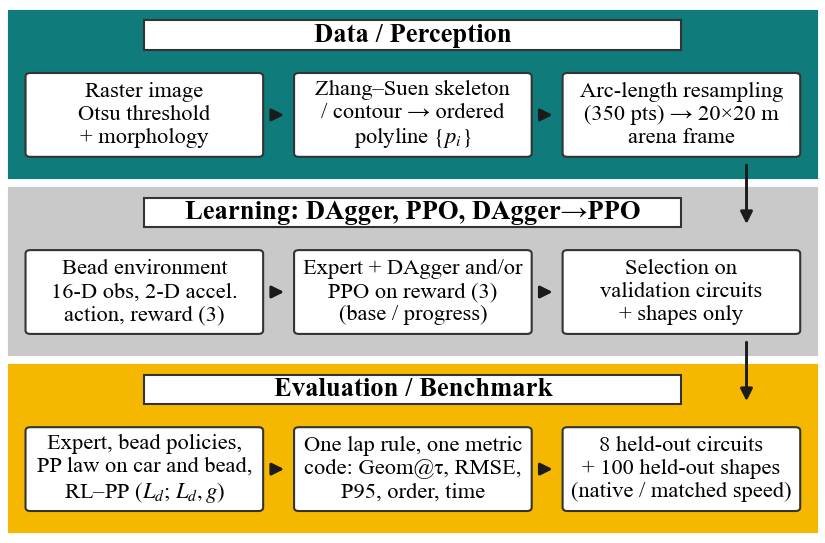
\includegraphics[width=\columnwidth]{fig1_pipeline.png}
\vskip -0.5pc
\caption{System overview: image to ordered reference path; bead network trained by DAgger, PPO or DAgger$\to$PPO with selection on validation paths; all controllers scored with one lap rule and one metric code on circuits and shapes kept out of training.}\label{fig:pipeline}
\vskip -1pc
\end{figure}
\subsection{Reference extraction}\label{sec:perception}
An input image is first reduced to at most 1200~px on its longer side, turned into gray scale and blurred with a Gaussian kernel. A global Otsu threshold~\cite{otsu1979} then splits stroke from background, with the polarity taken from the median gray level of the border pixels, and a $3\times3$ morphological closing removes small gaps. A drawing occupying no more than a fifth of the image is thinned to single-pixel width with the Zhang--Suen algorithm~\cite{zhang1984}; bigger regions are followed along their outer boundary. The pixels of each 8-connected skeleton piece are put in order by a walk that starts at one end and, at a branch, takes the neighbour with the smallest change of direction. After scaling to a $20\times20$~m arena, any piece under 0.1~m is discarded and the others share about 350 equally spaced points; no distance computation crosses the breaks between pieces. Images without a valid path are reported as failures, never replaced by a default path. Each circuit image is drawn from a centerline we know, which makes the extraction error directly measurable: per circuit, the extracted reference lies on average \VextMeanLo--\VextMeanHi~cm from the source centerline, and at most \VextMax~cm. Rasterization also shrinks the F1TENTH tracks by a linear factor of \VscaleLo--\VscaleHi\ (median \VscaleMed), to 39--82~m, and the spacing of the extracted waypoints is \VspMin--\VspMax~cm per circuit (median \VspMed~cm; Table~\ref{tab:spacing}). Four sample inputs and their paths appear in Fig.~\ref{fig:inputs}.

\begin{table}[t]
\caption{Waypoint spacing of the extracted circuit references (median and range of the distance between consecutive waypoints).}\label{tab:spacing}
\centering
\resizebox{\columnwidth}{!}{%
\setlength{\tabcolsep}{3pt}
\renewcommand{\arraystretch}{0.88}%
\begin{tabular}{llccc|llccc}
\toprule
Circuit & Split & $N$ & Median & Range & Circuit & Split & $N$ & Median & Range\\
 & & & [cm] & [cm] & & & & [cm] & [cm]\\
\midrule
\tabinput tables/tab_spacing_2col.tex
\bottomrule
\end{tabular}}
\par\vskip 2pt\parbox{\columnwidth}{\footnotesize$^\ddagger$Shortest segment is the last one, where the extracted loop stops short of its start and its final points hook back slightly; it is not a junction between pieces (no circuit reference has a break): Spielberg 5.6~cm, loop open by 8.2~cm, minimum of the other segments 15.7~cm; Austin 10.5~cm, loop open by 4.6~cm, minimum of the other segments 12.9~cm.
}
\end{table}

\begin{figure}[t]
\centering
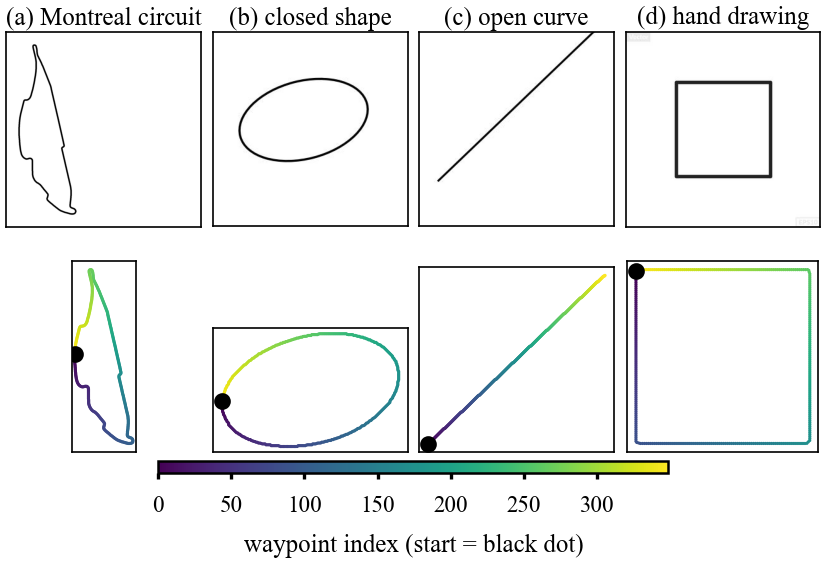
\includegraphics[width=\columnwidth]{fig8_inputs.png}
\vskip -0.5pc
\caption{From image to reference path. Upper row: four inputs, namely one test circuit rendered as an image, one closed and one open synthetic test contour, and a hand drawing. Lower row: the ordered paths obtained from them, shaded by waypoint number, with waypoint 0 shown as a black dot.}\label{fig:inputs}
\vskip -1pc
\end{figure}

\subsection{Bead dynamics, observation and reward}\label{sec:dyn}
The bead is modelled as a point mass with position $\mathbf{p}_t$, velocity $\mathbf{v}_t$ and command $\mathbf{u}_t\in[-1,1]^2$, scaled to at most $a_{\max}=10$~m/s$^2$ per axis, with viscous friction $\mu=7$~s$^{-1}$, $v_{\max}=7$~m/s and $\Delta t=0.016$~s:
\begin{equation}
\begin{aligned}
&\mathbf{v}_{t+1}=(\mathbf{v}_t+a_{\max}\mathbf{u}_t\Delta t)(1-\mu\Delta t),\\
&\mathbf{p}_{t+1}=\mathbf{p}_t+\mathbf{v}_{t+1}\Delta t.
\end{aligned}\label{eq:dyn}
\end{equation}
Full actuation along a single axis yields the steady speed $v^{*}=a_{\max}\Delta t(1-\mu\Delta t)/(\mu\Delta t)\approx1.27$~m/s. A waypoint counter $w_t$ may move ahead by four indices or fewer in one step, and only onto points closer than $\rho=0.18$~m; a lap is finished when $w_t$ reaches 99\% of the path, and episodes end after $\max(3500,\lceil1.5L/(v^{*}\Delta t)\rceil)$ steps for a path of length $L$ or after 400 steps without progress. The PP car uses the same counter code, lap rule, stall rule and step cap.

The policy observes 16 values scaled to $[-1,1]$ by construction (vectors to waypoints $w_t$, $w_t+1$ and $w_t+5$, position, velocity and heading, the distance to the path, an on-path flag, a curvature measure and the completed fraction), so no running input normalization is used. With $e_t$ the gap to the closest point of the reference, $d_t$ the gap to waypoint $w_t$, $n_t$ the waypoints passed in step $t$ and $\hat{\mathbf{r}}_t$ the path tangent, the reward is
\begin{align}
r_t={}&0.1\,\mathrm{clip}\big((d_{t-1}-d_t)/\rho,\pm1\big)+0.4\,n_t\nonumber\\
&+0.25\,e^{-(e_t/0.08)^2}+0.15\,\mathrm{clip}(\mathbf{v}_t\!\cdot\hat{\mathbf{r}}_t/v_{\max},\pm1)\nonumber\\
&-0.05\min(e_t/0.1,3)-0.1\cdot\mathbf{1}[e_t>\rho]\nonumber\\
&-0.05\cdot\mathbf{1}_{\mathrm{back}}-0.5\cdot\mathbf{1}_{\mathrm{wall}}\nonumber\\
&-0.005\min(\|\mathbf{u}_t-\mathbf{u}_{t-1}\|,1)-0.001,\label{eq:reward}
\end{align}
plus $+50$ for a finished lap, $+15$ for a truncated episode past 80\% and $-5$ otherwise; the weights were set before the data split and not tuned. Because every step pays the centering bonus, a slower lap earns more of it: adding Gaussian noise of standard deviation \VexStd\ to the expert's actions triples its validation RMSE (\VexRmseZero\ to \VexRmseNoise~cm) yet raises its return from \VexRewBzero\ to \VexRewBnoise. A \emph{progress} variant therefore pays the bonus per waypoint passed, $2.0\,n_t e^{-(e_t/0.08)^2}$, keeping its per-lap budget at the expert's pace; the noisy expert then earns less than the noise-free one (\VexRewPnoise\ versus \VexRewPzero).

\subsection{Learning the bead controller}\label{sec:learning}
All bead policies share one actor--critic architecture, implemented in Stable-Baselines3~\cite{raffin2021}: actor and critic are separate two-layer tanh networks with 256 units per layer, and actions are sampled from a Gaussian with state-independent spread. During testing the mean action is executed. The hand-written \emph{expert} steers toward the next waypoint,
\begin{equation}
\mathbf{u}^{*}_t=(\mathbf{p}[w_t+1]-\mathbf{p}_t)/\|\mathbf{p}[w_t+1]-\mathbf{p}_t\|.\label{eq:expert}
\end{equation}

\textbf{Bead-DAgger} first regresses the actor on a single teacher episode for each training path and refines it with DAgger (Algorithm~\ref{alg:dagger}); the reward is not used. The teacher is the expert (\ref{eq:expert}) or, in \emph{Bead-DAgger (Bead-PP teacher)}, the PP law run on the bead (Section~\ref{sec:beadpp}).

\textbf{Bead-PPO} trains the same network from a random initialization by maximizing the clipped PPO objective,
\begin{equation}
\begin{aligned}
\mathcal{L}(\theta)={}&\mathbb{E}_t\big[\min(\varrho_t\hat A_t,\mathrm{clip}(\varrho_t,1\pm\epsilon)\hat A_t)\big]\\
&-c_v\mathcal{L}^{V}+c_e\mathcal{H},
\end{aligned}\label{eq:ppo}
\end{equation}
with GAE advantages~\cite{schulman2016}, for $3\times10^6$ steps. The starting value $\log\sigma_0=-0.5$ of the policy's log standard deviation was picked among $\{-1,-0.5,0\}$ by a pilot with seed 100 scored on validation references only (scores \VpilotPmscore, \VpilotPhscore\ and \VpilotPzscore\ after $7.5\times10^5$ steps).

\textbf{Bead-DAgger$\to$PPO} starts from the expert-taught DAgger actor with the same seed, holds that actor fixed for $5\times10^4$ steps while only the critic learns, and continues with (\ref{eq:ppo}) for $2\times10^6$ steps. To avoid scrambling the initial policy it starts with $\log\sigma_0=-2$, uses the learning rate $10^{-4}$, and adds a behaviour-cloning term
\begin{equation}
\mathcal{L}_{\mathrm{BC}}(\theta)=\lambda\,\mathbb{E}_t\big[\|\boldsymbol{\mu}_\theta(\mathbf{o}_t)-\mathbf{u}^{*}_t\|^2\big],\quad\lambda=1,\label{eq:bc}
\end{equation}
where $\boldsymbol{\mu}_\theta$ is the actor mean and $\mathbf{u}^{*}_t$ is recovered exactly from the observation. Both PPO procedures are run with the base and the progress reward.

Each variant learns on the training split, and its final checkpoint is the one scoring highest on validation; the score is average Geom@0.10 (as a fraction) less average RMSE (in meters), averaged over validation circuits and shapes. In these units 1~cm of RMSE weighs as much as one percentage point of coverage; RMSE alone does not notice skipped sections, which Geom@0.10 penalizes. Selecting by RMSE alone would have chosen the same checkpoint or setting in \VselSame\ of \VselTotal\ runs and grids, and otherwise a validation RMSE within \VselMaxDiff~cm. Hyper-parameters are listed in Table~\ref{tab:hyper}.

\begin{table}[t]
\caption{Learning hyper-parameters.}\label{tab:hyper}
\centering
\resizebox{\columnwidth}{!}{%
\setlength{\tabcolsep}{2pt}
\renewcommand{\arraystretch}{0.88}%
\begin{tabular}{lll}
\toprule
Quantity & Bead (PPO variants) & RL--PP (adaptation of~\cite{elgouhary2026})\\
\midrule
MLP (policy/value) & $[256,256]$ tanh & $[64,64]$ tanh\\
$n_{\mathrm{steps}}$ / batch / epochs & 2048$\times$4 envs / 128 / 10 & 2048 / 256 / 5\\
$\gamma$ / GAE $\lambda$ / clip & 0.99 / 0.95 / 0.2 & 0.99 / 0.98 / 0.2 (KL 0.015)\\
Entropy / value coeff. & 0.001 / 0.5 & 0.02 / 0.6\\
Learning rate & $3\!\times\!10^{-4}$; fine-tune $10^{-4}$ & $2.4\!\times\!10^{-4}$, linear decay\\
Initial $\log\sigma$ & $-0.5$; fine-tune $-2$ & 0\\
BC weight $\lambda$ & fine-tune 1 (check: 0.1, 10) & --\\
Normalization & none (inputs in $[-1,1]$) & VecNormalize (obs., return)\\
Steps per run & $3\!\times\!10^6$; fine-tune $2\!\times\!10^6$ & $10^5$\\
Training seeds & 0--4 & 0--4\\
\bottomrule
\end{tabular}}
\end{table}

\begin{algorithm}[t]
\caption{DAgger for the bead (Bead-DAgger).}
\label{alg:dagger}
\begin{algorithmic}[1]
\STATE \textbf{Input:} training paths $\mathcal{T}$, validation paths $\mathcal{V}$, teacher $\pi^{*}$, network $\pi_\theta$, $\beta=(0.4,0.2,0.1,0.05,0,0,0,0)$
\STATE $\mathcal{D}\leftarrow$ one teacher episode per $\tau\in\mathcal{T}$; fit actor on $\mathcal{D}$ (12 epochs, lr $2\times10^{-4}$)
\FOR{round $k=1,\dots,8$}
\STATE for each $\tau\in\mathcal{T}$ roll out one episode; \emph{at every step} execute $\pi^{*}$ with probability $\beta_k$, else $\pi_\theta$, and label the state with $\pi^{*}(o)$
\STATE $\mathcal{D}\leftarrow\mathcal{D}\cup\{(o,\pi^{*}(o))\}$; refit actor (8 epochs, lr $1.5\times10^{-4}$ for $k\le3$, else $7\times10^{-5}$)
\STATE keep the checkpoint if the validation score on $\mathcal{V}$ improves
\ENDFOR
\STATE \textbf{return} best validation checkpoint
\end{algorithmic}
\end{algorithm}

\subsection{Pure Pursuit baselines}\label{sec:rlpp}
The PP car is a kinematic bicycle~\cite{rajamani2012} with wheelbase $W=0.33$~m. With $y'$ the sideways offset, in the car's frame, of the lookahead point,
\begin{equation}
\begin{aligned}
&\gamma=g\cdot2y'/L_d^2,\qquad \dot\theta=(v/W)\tan\delta,\\
&\delta=\mathrm{clip}(\arctan(W\gamma),\pm1.10~\mathrm{rad}).
\end{aligned}\label{eq:pp}
\end{equation}
Speed follows $v_{\mathrm{ref}}=\mathrm{clip}(4.2/\sqrt{1+2.5|\kappa|},1.8,5.0)$~m/s with braking and acceleration passes. The model has no tyre forces: at native speed, tuned PP demands more than 10~m/s$^2$ of lateral acceleration in \VlatAccFrac\% of its test steps, which a real car could not sustain; at the matched speed below, the maximum is \VlatAccMaxM~m/s$^2$.

\textbf{Fixed and Adaptive PP} use constant $(L_d,g)$ and $L_d=\mathrm{clip}(a+bv,0.05,1.20)$ with $g=1.05$. Both are tuned by grid search over the training references, using the selection score above, over $L_d\in\{0.05,0.075,\dots,0.20\}\cup\{0.25,0.30,\dots,1.00\}$~m, $g\in\{0.6,\dots,1.4\}$, $a\in\{0,0.025,\dots,0.5\}$ and $b\in\{0,0.025,0.05,\dots,0.25\}$~s. Fixed PP selects $(\VfixL\ \mathrm{m},\VfixG)$ at native and $(\VfixLm\ \mathrm{m},\VfixGm)$ at matched speed, inside the grid (training RMSE \VtuneRa, \VtuneRb\ and \VtuneRc~cm at 0.10, 0.125 and 0.15~m). Adaptive PP selects $(a,b)=(\VadA,\VadB)$, but the best constant lookahead scores within 0.001~cm, so it is in effect a Fixed PP.

\textbf{Stanley}~\cite{hoffmann2007} runs on the same car: $\delta=\psi_{\mathrm{path}}-\psi+\arctan\big(k\,e_f/(k_s+v)\big)$, clipped to $\pm1.10$~rad, where $e_f$ is the signed distance of the front axle from the nearest path segment and $\psi_{\mathrm{path}}$ that segment's heading. Its gains are grid-searched with the same references, score and completion rule as PP, over $k\in\{0.25,\dots,4096\}$ and $k_s\in\{0.005,\dots,4\}$~m/s (\VstNgrid\ settings; smaller grids had their optimum on the edge and were widened until it lay inside). It selects $(k,k_s)=(\VstK,\VstKs)$ at native and $(\VstKm,\VstKsm)$ at matched speed, both inside the grid; from $k=512$ upward the score changes by less than 0.001.

\textbf{RL--PP} adapts~\cite{elgouhary2026}, an arXiv preprint that has not been peer reviewed, to our arena. A PPO agent observes speed, the curvature at the current waypoint and at those 5 and 12 ahead, their difference, the lateral error and the heading error, and outputs $L_d\in[0.05,1.20]$~m and $g\in[0.60,1.40]$, low-pass filtered with factor 0.2. Its reward follows the structure of~\cite{elgouhary2026}: distance from a teacher $L^{*}=\mathrm{clip}(0.65+0.04v-0.18\kappa_{\max},0.26,0.85)$, $g^{*}=\mathrm{clip}(0.96+0.14\kappa_{\max},0.6,1.4)$, parameter-change penalties, a bend term, progress, speed, wall and stall terms, plus a corridor bonus, a quadratic error penalty and an alignment bonus. Table~\ref{tab:adapt} lists every change; a separately trained $L_d$-only agent ($g=1.05$) serves as an ablation.

\begin{table}[t]
\caption{RL-tuned PP: original~\cite{elgouhary2026} and our adaptation.}\label{tab:adapt}
\centering
\resizebox{\columnwidth}{!}{%
\setlength{\tabcolsep}{2pt}
\renewcommand{\arraystretch}{0.88}%
\begin{tabular}{lll}
\toprule
Aspect & \cite{elgouhary2026} & This work\\
\midrule
Track scale & F1TENTH maps & shrunk \VscaleLo--\VscaleHi$\times$, $20\times20$~m\\
$L_d$ / $g$ range & $[0.35,4.0]$~m / $[0.45,1.15]$ & $[0.05,1.20]$~m / $[0.60,1.40]$\\
Teacher $L^{*}$ & $0.50+0.28v-3.5\kappa_{\max}$ & $0.65+0.04v-0.18\kappa_{\max}$\\
Teacher $g^{*}$ & decreasing in $v$ & increasing in $\kappa_{\max}$\\
Observations & $v,\kappa_{0,1,2},\Delta\kappa$ & + lateral and heading error\\
Reward & 11 weighted terms & own weights; no $|\kappa|$ term;\\
 & & + corridor, error, alignment terms\\
Speed profile & raceline, $\le$15.6~m/s & friction-limited, 1.8--5~m/s\\
Steering limit & PP command $\pm0.35$ & $|\delta|\le1.10$~rad\\
Training data & Hockenheim & 11 circuits + 120 contours\\
Budget & $\le1.2\times10^{6}$ steps, Optuna & $10^{5}$ steps, no tuning\\
Evaluation & simulation + 1:10 car & simulation only\\
\bottomrule
\end{tabular}}
\end{table}

\subsection{Pure Pursuit on the bead}\label{sec:beadpp}
\emph{Bead-PP} runs the car's Fixed PP law on the bead. With the same nearest-point window and lookahead search as the car and the heading taken from the bead's velocity, the curvature $\gamma$ of (\ref{eq:pp}) is applied as a lateral acceleration $v^2\gamma$; a longitudinal acceleration, obtained by inverting one step of (\ref{eq:dyn}), holds the speed at $v_{\mathrm{match}}$, and steering has priority when $a_{\max}$ is reached. Bead-PP is tuned on the same grid and references as the car and selects $(\VbppL\ \mathrm{m},\VbppG)$, inside the grid. As a second control, the expert (\ref{eq:expert}) aims at waypoint $w_t+k$, $k=1,\dots,10$, anchored on $w_t$ or on the tracked nearest point; the best $k$ is selected on training references.

\section{Experimental Setup}
\subsection{Data, protocol and metrics}
We rasterized and extracted every one of the 23 circuits in the public F1TENTH racetrack collection. The test split receives Hockenheim, Montreal and Yas Marina; a seeded permutation chosen ahead of training divides the remaining 20 into 11 training, 4 validation and 5 additional test circuits (Fig.~\ref{fig:split}). Two synthetic sets of 1000 images, one of closed shapes (polygons, ellipses, rounded quadrilaterals) and one of open curves (arcs, lines, parabolas), add 60 training references each; 25 per set serve checkpoint selection, and the first 50 in each set are test cases. Because all synthetic images come from one generator, they measure generalization within that distribution, whereas the held-out circuits measure transfer to new layouts. In total \VnRefs\ references were extracted without failure.

\begin{figure}[t]
\centering
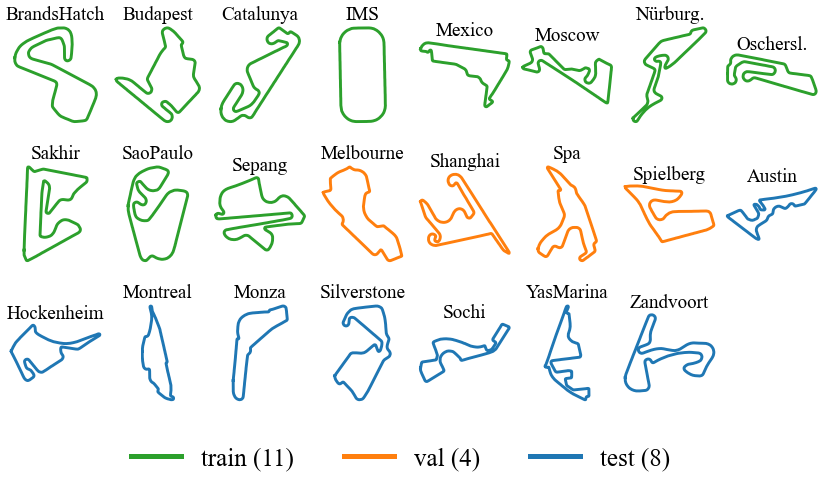
\includegraphics[width=\columnwidth]{fig2_split.png}
\vskip -0.5pc
\caption{The 23 extracted F1TENTH references, with color indicating the split. Besides the three circuits that trained the naive-protocol bead (Yas Marina, Montreal, Hockenheim), five more form the test set; none of them is used to train, tune or select any controller.}\label{fig:split}
\vskip -1pc
\end{figure}

Each controller drives every test circuit five times (start perturbed by up to $\pm5$~cm) and every test contour once, deterministically. Learned controllers have five training seeds (three in the behaviour-cloning weight check). In Track~A each controller drives at its own pace; in Track~B the target speed of the car may not exceed $v_{\mathrm{match}}=1.256$~m/s, the expert's mean speed on the training circuits, and PP is tuned and RL--PP trained again at this speed; Bead-PP runs at $v_{\mathrm{match}}$. Counting training seeds separately, \VnInst\ controller instances ran \VnEpisodes\ test episodes. Every metric was recomputed from the stored trajectories, partly with independent code, and re-running \VnRerun\ instances from their saved checkpoints reproduced the trajectories bit for bit.

All distances are to \emph{polylines}, not to points. With $\mathcal{P}$ the set of reference points, $P$ the polyline through them and $X$ the trajectory polyline, the tracking error of sample $\mathbf{x}_t$ is $e(\mathbf{x}_t)=\mathrm{dist}(\mathbf{x}_t,P)$, which yields the RMSE, the largest error and the error's 95th percentile (P95); coverage counts the reference points lying at most $\tau$ from the trajectory polyline,
\begin{equation}
\mathrm{Geom@}\tau=\frac{1}{|\mathcal{P}|}\sum_{\mathbf{p}\in\mathcal{P}}\mathbf{1}\big[\mathrm{dist}(\mathbf{p},X)\le\tau\big].\label{eq:geom}
\end{equation}
Ordered coverage is the size of the biggest group of reference points reached ($\le\rho$) in path order, computed by dynamic programming; a run with ordered coverage of at least 0.95 is completed. The same code scores every controller, against the extracted reference and, for the circuits, against the true centerline. Under a \emph{naive protocol} we also score a bead fitted to the expert by regression, with its checkpoint chosen on Hockenheim, Montreal and Yas Marina, an RL--PP agent trained on just one hand-drawn contour and run without its normalization statistics, and PP with hand-set gains $(0.55\ \mathrm{m},1.05)$ and $(a,b)=(0.35,0.25)$; these rows enter no comparison.

\textbf{Statistics.} Every comparison pairs the two controllers circuit by circuit on the 8 test circuits, after averaging seeds and episodes. The main evidence is the mean difference and its bootstrap interval at the 95\% level (10\,000 resamples of circuits, and of seeds within learned controllers). With $n=8$, an exact signed-rank Wilcoxon test cannot give $p<0.0078$, which requires all circuits to agree, so only four primary RMSE comparisons are tested, with Holm correction: (P1) Bead-DAgger versus Fixed PP at $v_{\mathrm{match}}$; (P2) Bead-DAgger$\to$PPO versus Bead-DAgger; (P3) RL--PP joint versus Fixed PP; (P4) Bead-PP versus the expert. They were declared before the final evaluation; a preliminary run of Bead-PP and of the expert sweep had, however, touched the test circuits before the settings were fixed (no setting was chosen from it). Other comparisons are exploratory. Episodes are not pooled, since those on one circuit differ only by the start perturbation.

\section{Results and Discussion}

\begin{table*}[t]
\caption{Accuracy against the extracted references on the eight unseen test circuits, averaged over circuits with five episodes per circuit. Learned controllers: average of five training seeds (three for $\lambda=10$), with the seed range in brackets. Bold: most accurate entry of each column.}\label{tab:circuits}
\centering
\resizebox{\textwidth}{!}{%
\setlength{\tabcolsep}{3pt}
\renewcommand{\arraystretch}{0.88}%
\begin{tabular}{lccccccccc}
\toprule
Controller & Geom@0.05 [\%] & Geom@0.10 [\%] & RMSE [cm] & P95 [cm] & Max [cm] & Ordered [\%] & Completed [\%] & Time [s] & Speed [m/s]\\
\midrule
\tabinput tables/tab_circuits.tex
\bottomrule
\multicolumn{10}{l}{$^\ast$Naive protocol: actor regressed onto the expert and selected on three of the eight test circuits (Yas Marina, Montreal, Hockenheim).}\\
\multicolumn{10}{l}{$^\dagger$Naive protocol: trained on just one hand-drawn contour; run on raw observations. $^\S$The Fixed PP law executed on the bead at $v_{\mathrm{match}}$.}
\end{tabular}}
\end{table*}

\subsection{Accuracy on held-out circuits}
Table~\ref{tab:circuits} gives the results against the extracted references. \textbf{Bead-DAgger matches its expert} (\VrmseDagger\ versus \VrmseExpert~cm) with almost no spread across seeds. All PPO-trained variants are less accurate: Bead-DAgger$\to$PPO reaches \VrmseDP~cm (\VrmseDPacc~cm with the progress reward) while scratch-trained Bead-PPO reaches \VrmsePPO~cm (\VrmsePPOacc~cm), completing \VcompPPO\% (\VcompPPOacc\%) of its test runs. \textbf{Against these references, tuned Fixed PP is more accurate than every learned bead controller}, including the one taught by PP (Section~\ref{sec:plant}): it reaches \VrmseFix~cm at native speed and \VrmseFixM~cm at $v_{\mathrm{match}}$, and tuned Adaptive PP reaches \VrmseAd~cm; RL--PP reaches \VrmseRL~cm (joint) and \VrmseRLld~cm ($L_d$ only). Fig.~\ref{fig:bars} summarizes accuracy and spread across seeds. Because both plants share the lap rule, Geom@0.10 is equal for every controller that completes its laps. Hand-set Adaptive PP completes no lap: its lookahead of 0.8--1.6~m cuts corners by more than $\rho$. \textbf{Tuned Stanley is less accurate than PP at the car's reference point}: \VrmseSt~cm at native and \VrmseStM~cm at matched speed, behind Fixed PP on every circuit (\VcmpStFixMDiff~cm [\VcmpStFixMLo, \VcmpStFixMHi] at $v_{\mathrm{match}}$; \VtrueStFixMDiff~cm against the true centerlines), and it completes \VcompSt\% of its runs: at one Montreal hairpin its rear axle passes about 20~cm from the path, beyond the lap counter's radius $\rho$, and the run stops after 400 steps without progress. This follows from what each law regulates: Stanley steers the front axle onto the path, so the rear axle cuts corners by about $W^2/(2R)$ for a corner of radius $R$, whereas PP steers the rear axle. At the front axle the order reverses (\VfrontStM~cm for Stanley, \VfrontFixM~cm for Fixed PP at $v_{\mathrm{match}}$). The car's position and all metrics refer to the rear axle, so PP is the matching geometric law here, and our results on tuned geometric control refer to PP.

Fig.~\ref{fig:traces} shows complete laps on three test circuits, and Fig.~\ref{fig:cdf} the error distribution across the test circuits: under the PP law, \VwithinBpp\% (Bead-PP), \VwithinFix\% (Fixed PP) and \VwithinAd\% (Adaptive PP) of all samples lie closer than 3~cm to the reference, compared with \VwithinExpert\% for the expert, \VwithinDagger\% for Bead-DAgger, \VwithinRL\% for RL--PP, \VwithinDP\% for Bead-DAgger$\to$PPO and \VwithinPPO\% for Bead-PPO. The failures of the bead policies are visible in Fig.~\ref{fig:zoom}: at the two Montreal corners with the largest Bead-DAgger$\to$PPO miss, that policy leaves by a small margin the almost common line of tuned Fixed PP, RL--PP, the expert and Bead-DAgger, while scratch-trained Bead-PPO drives inside the corner.

\begin{figure}[t]
\centering
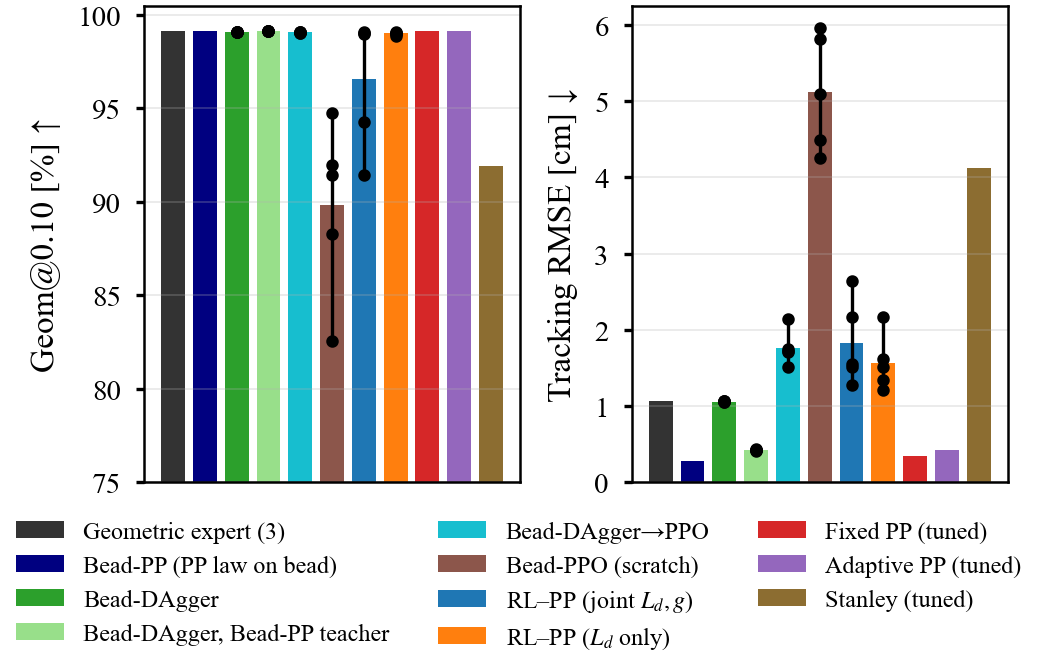
\includegraphics[width=\columnwidth]{fig3_bars.png}
\vskip -0.5pc
\caption{Test-circuit averages: Geom@0.10 on the left (higher is better), RMSE on the right (lower is better). Dots mark the individual training seeds of the learned controllers.}\label{fig:bars}
\vskip -1pc
\end{figure}

\begin{figure}[t]
\centering
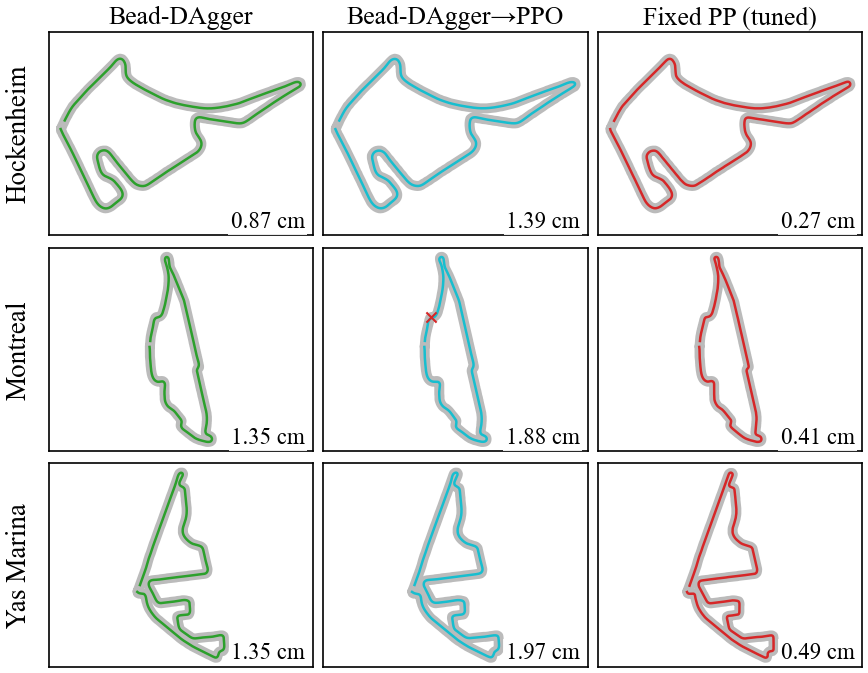
\includegraphics[width=\columnwidth]{fig9_traces.png}
\vskip -0.5pc
\caption{Complete laps (first episode, seed 0) drawn over the grey reference on three unseen circuits. A red cross marks a reference point missed by more than 0.10~m (the start/finish join is ignored); the number in each panel is the RMSE of that lap.}\label{fig:traces}
\vskip -1pc
\end{figure}

\begin{figure}[t]
\centering
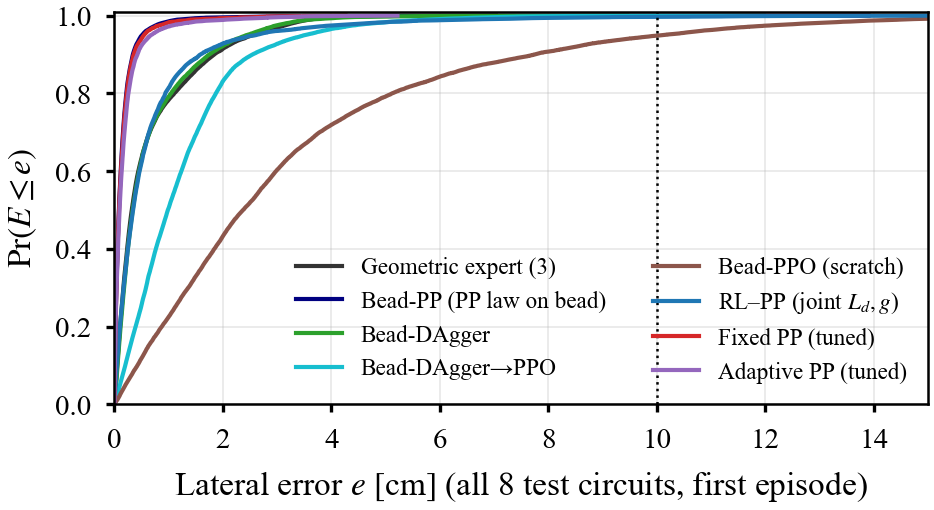
\includegraphics[width=\columnwidth]{fig11_cdf.png}
\vskip -0.5pc
\caption{Fraction of trajectory samples whose distance to the extracted reference stays below a threshold, with all eight test circuits taken together (first episode; seed 0 for learned controllers). The dotted line is at 0.10~m.}\label{fig:cdf}
\vskip -1pc
\end{figure}

\begin{figure}[t]
\centering
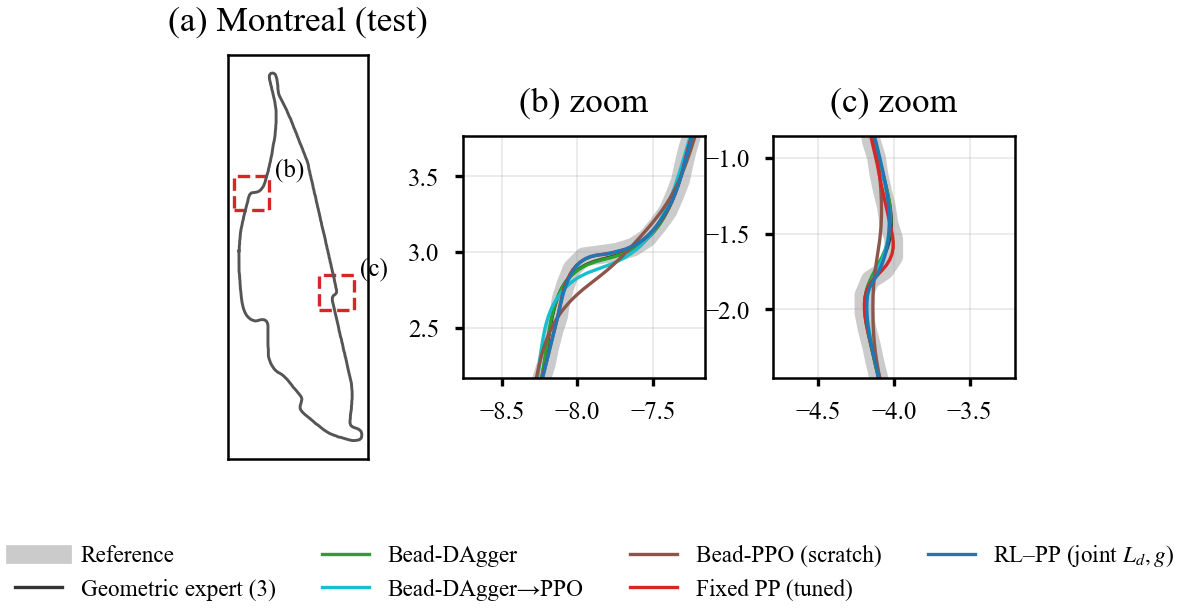
\includegraphics[width=\columnwidth]{fig6_zoom.png}
\vskip -0.5pc
\caption{Close-up of the controllers on the unseen Montreal circuit (first episode, seed 0). Both zoom windows are placed by the script at the two reference points where Bead-DAgger$\to$PPO strays furthest, leaving out the start/finish area.}\label{fig:zoom}
\vskip -1pc
\end{figure}

\textbf{Measured against the true centerlines} (Table~\ref{tab:truecl}), every error grows by the extraction error, and the differences between good controllers shrink. The gap between Bead-DAgger and Fixed PP at $v_{\mathrm{match}}$ falls from \VcmpPoneDiff\ [\VcmpPoneLo, \VcmpPoneHi]~cm to \VtruePoneDiff\ [\VtruePoneLo, \VtruePoneHi]~cm, and that between Bead-PP and the expert from \VcmpPfourDiff\ to \VtruePfourDiff~cm. These gaps are of the size of the extraction error itself (\VextMeanLo--\VextMeanHi~cm), but they keep their sign on all eight circuits, all four primary intervals still exclude zero, and the ranking of all controllers is nearly unchanged (rank correlation \VrankCorr).

\begin{table}[t]
\caption{RMSE against the extracted references and RMSE, P95 and Geom@0.10 against the true F1TENTH centerlines (eight test circuits).}\label{tab:truecl}
\centering
\resizebox{\columnwidth}{!}{%
\setlength{\tabcolsep}{3pt}
\renewcommand{\arraystretch}{0.88}%
\begin{tabular}{lcccc}
\toprule
 & Extracted & \multicolumn{3}{c}{True centerline}\\
Controller & RMSE & RMSE & P95 & G@0.10\\
 & [cm] & [cm] & [cm] & [\%]\\
\midrule
\tabinput tables/tab_truecl.tex
\bottomrule
\end{tabular}}
\end{table}

\subsection{Control law, vehicle and teacher}\label{sec:plant}
\textbf{The control law, not the vehicle, explains the gap.} On the bead at $v_{\mathrm{match}}$ the PP law reaches \VrmseBpp~cm, as accurate as on the equally fast car and below the expert on all eight circuits (P4). On the training circuits its error depends on $L_d$ in the same way on both plants, with the same optimum (Fig.~\ref{fig:plant}, left), so the bead is not harder to steer accurately. Aiming the expert further ahead does not help (Fig.~\ref{fig:plant}, right): the best target is the next waypoint ($k=\VekSelC$, \VekRmseC~cm), or $k=\VekSelN$ with the nearest-point anchor (\VekRmseN~cm), and from $k=\VekFailC$ on laps are no longer completed. Unlike PP, the expert does not turn the offset of its target into a curvature command.

\textbf{The teacher, more than the network, limited the imitation policy.} Taught by Bead-PP instead of the expert, with the same Algorithm~\ref{alg:dagger}, Bead-DAgger reaches \VrmseDaggerBpp~cm: \VcmpBppDagDiff~cm [\VcmpBppDagLo, \VcmpBppDagHi] relative to the expert-taught policy, better on all eight circuits. Against the extracted references it stays \VcmpBppTeachDiff~cm [\VcmpBppTeachLo, \VcmpBppTeachHi] behind its teacher and \VcmpBppFixMDiff~cm [\VcmpBppFixMLo, \VcmpBppFixMHi] behind tuned PP on the equally fast car, on every circuit. Against the true centerlines both differences vanish: \VtrueBppTeachDiff~cm [\VtrueBppTeachLo, \VtrueBppTeachHi] relative to its teacher and \VtrueBppFixMDiff~cm [\VtrueBppFixMLo, \VtrueBppFixMHi] relative to tuned PP (Table~\ref{tab:truecl}). The network can therefore represent a controller as accurate as tuned PP on the real track, but by imitation it approaches, and does not exceed, its teacher.

\begin{figure}[t]
\centering
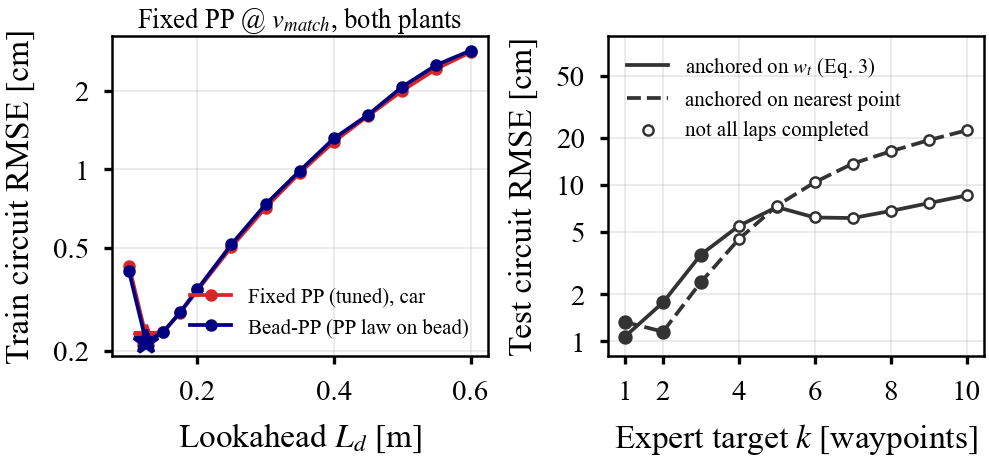
\includegraphics[width=\columnwidth]{fig12_bead_pursuit.png}
\vskip -0.5pc
\caption{Left: training-circuit RMSE of the same Fixed PP law on the car and on the bead at $v_{\mathrm{match}}$ versus $L_d$ (best gain per $L_d$; star: selected). Right: test-circuit RMSE of the expert aiming $k$ waypoints ahead; open markers: not every lap completed.}\label{fig:plant}
\vskip -1pc
\end{figure}

\subsection{How PPO changes the bead policy}\label{sec:ppo}
PPO changes the actor, the critic and the action noise (unit tests; with the actor frozen for the critic's warm-up the approximate KL divergence \VfrozenKL); at the end of training the approximate KL per update is \VklLo--\VklHi\ and the explained variance \VevLo--\VevHi. PPO from scratch improves slowly and remains far from the expert after $3\times10^6$ steps (Fig.~\ref{fig:learning}). Fine-tuning moves away from the DAgger policy despite the small initial noise, the lower learning rate and the behaviour-cloning term, and raised the test RMSE on all eight circuits for both rewards (P2). Ranked by base reward on the test circuits, the noise-free policies come out in the same order as by accuracy: the expert collects \VrewExpert, Bead-DAgger \VrewDagger, Bead-DAgger$\to$PPO \VrewDP\ and Bead-PPO \VrewPPO. PPO, however, optimizes a stochastic policy, so each policy also drove the four circuits of the validation split, both with and without Gaussian noise on its actions (three noise seeds, five training seeds). With the base reward, deterministic Bead-DAgger earns \VdiagDPDagDetrew\ (RMSE \VdiagDPDagDetrmse~cm) and, with the initial fine-tuning noise, \VdiagDPDagStorew\ (\VdiagDPDagStormse~cm); the fine-tuned policy obtains \VdiagDPFtStorew\ under its own noise ($\sigma\approx\VdiagDPStdEnd$) and \VdiagDPFtDetrew\ noise-free (\VdiagDPFtDetrmse~cm). With the progress reward the returns are \VdiagDPaccDagDetrew\ and \VdiagDPaccDagStorew\ before and \VdiagDPaccFtStorew\ and \VdiagDPaccFtDetrew\ after fine-tuning (\VdiagDPaccFtDetrmse~cm deterministic). Fine-tuning thus lowered the return of the stochastic policy it optimizes, under either reward, so the drop in accuracy cannot be explained by training a noisy policy and testing a noise-free one. With the progress reward the bead became faster and less accurate. A check of the behaviour-cloning weight (seeds 0--2, base reward, selection on validation only) gave mean validation RMSEs of \VbcValLow, \VbcValOne\ and \VbcValHigh~cm for $\lambda=0.1$, 1 and 10, against \VbcValDagger~cm for the DAgger policy. With the selected $\lambda=\VbcSel$, the fine-tuned policy reaches \VrmseDPbcHigh~cm on the test circuits: less degraded than with $\lambda=1$, but still \VcmpBcDagDiff~cm [\VcmpBcDagLo, \VcmpBcDagHi] behind its starting point. Which factor---the critic, the mix of long circuits and short contours, the step size or the budget---causes the degradation was not isolated: \textbf{with our PPO budget and settings, PPO did not improve the imitation policy}.

\begin{figure}[t]
\centering
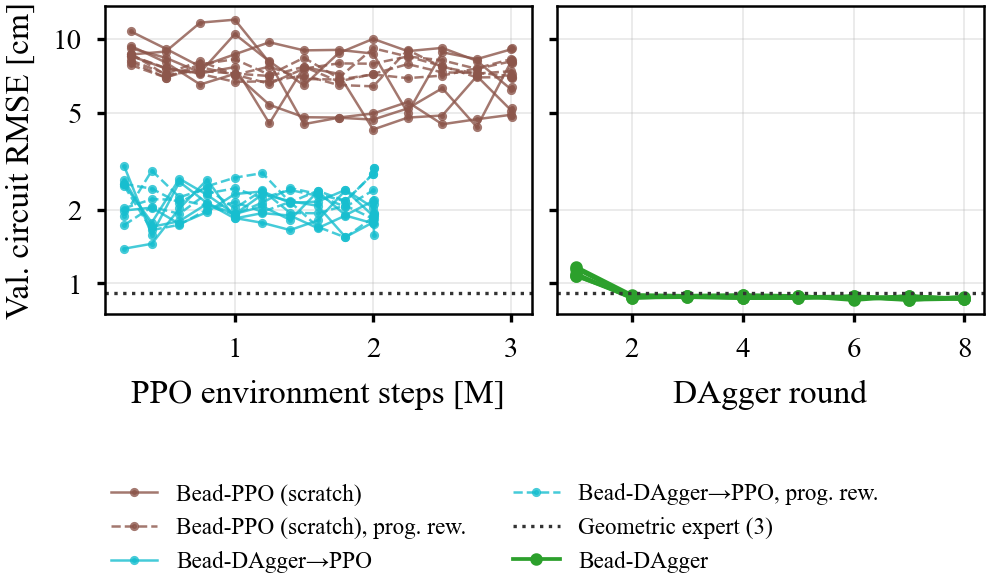
\includegraphics[width=\columnwidth]{fig5_learning.png}
\vskip -0.5pc
\caption{RMSE on the validation circuits as training proceeds (five seeds). Left: PPO from random initial weights and PPO from the DAgger actor, with the base (solid) and progress (dashed) reward. Right: the eight DAgger rounds (expert teacher). Dotted: expert.}\label{fig:learning}
\vskip -1pc
\end{figure}

\subsection{Naive protocol, speed and contours}\label{sec:naiveres}
On its own training circuits (Hockenheim, Montreal, Yas Marina) the naive bead reaches \VthreePubBeadLo--\VthreePubBeadHi~cm, against \VthreeFixOrigLo--\VthreeFixOrigHi~cm for PP with hand-set gains and \VthreePubRLLo--\VthreePubRLHi~cm for naive RL--PP, so on each circuit direct actuation appears the most precise of the three (Table~\ref{tab:paper}). However, tuned PP reaches \VthreeFixLo--\VthreeFixHi~cm on the same circuits and the expert that the naive bead imitates \VthreeExpertLo--\VthreeExpertHi~cm. Over all eight test circuits, Fixed PP with hand-set gains reaches \VrmseFixOrig~cm and naive RL--PP \VrmsePubRL~cm. The naive bead averages \VthreePubBeadMean~cm on its training circuits but \VrestPubBead~cm on the five unseen ones: untuned baselines reverse the ranking, and leakage inflates the learned controller.

\begin{table}[t]
\caption{Scores on the three circuits that trained the naive-protocol bead, as Geom@0.10 [\%] and RMSE [cm]; bold marks the best entry per column.}\label{tab:paper}
\centering
\resizebox{\columnwidth}{!}{%
\setlength{\tabcolsep}{2.5pt}
\renewcommand{\arraystretch}{0.88}%
\begin{tabular}{lcccccc}
\toprule
& \multicolumn{2}{c}{Hockenheim} & \multicolumn{2}{c}{Montreal} & \multicolumn{2}{c}{Yas Marina}\\
Controller & G@0.10 & RMSE & G@0.10 & RMSE & G@0.10 & RMSE\\
\midrule
\tabinput tables/tab_paper_circuits.tex
\bottomrule
\end{tabular}}
\end{table}

Driving at its own pace, the bead needs about 2.3 times the car's lap time (\VtExpert\ versus \VtFix~s, Fig.~\ref{fig:pace}), as friction caps its speed at roughly 1.3~m/s, whereas the car's speed profile peaks at 5~m/s on straight segments. At $v_{\mathrm{match}}$ the car's lap time nearly equals the bead's (\VtFixM\ versus \VtExpert~s) and its error drops slightly, to \VrmseFixM~cm for re-tuned Fixed PP and \VrmseAdM~cm for Adaptive PP, while retrained RL--PP reaches \VrmseRLM~cm; tuned PP is still the more accurate (P1).

\begin{figure}[t]
\centering
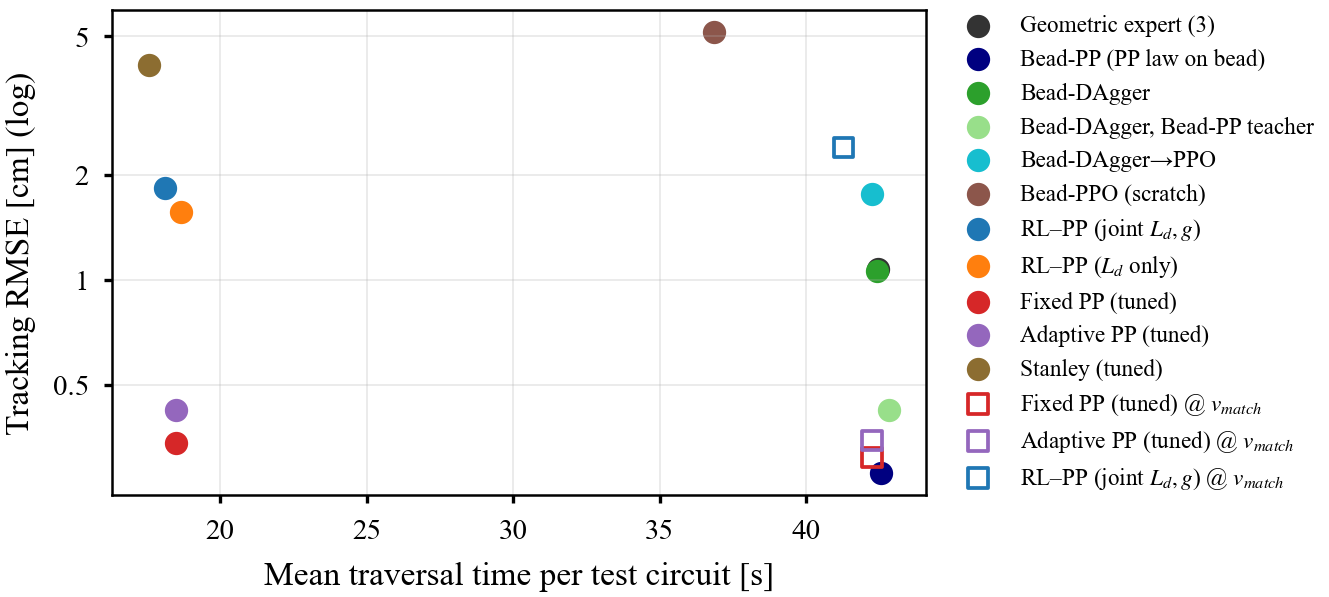
\includegraphics[width=\columnwidth]{fig4_pace.png}
\vskip -0.5pc
\caption{Accuracy against lap time on the test circuits. Solid circles: every controller at its own speed (Track~A). Hollow squares: the car's PP-family controllers with their target speed limited to $v_{\mathrm{match}}$ (Track~B).}\label{fig:pace}
\vskip -1pc
\end{figure}

\textbf{Dynamic vehicle model.} To check whether the kinematic car flatters PP, the car controllers were also run at $v_{\mathrm{match}}$ on the dynamic single-track model with linear tyres of F1TENTH Gym~\cite{okelly2020} (its mass, inertia, axle distances, cornering stiffnesses and switch to kinematics below 0.5~m/s; position at the rear axle; steering limit kept at $\pm1.10$~rad, as arena hairpins need about 1~rad), (a) with the tyres alone and (b) also with its steering-rate limit of 3.2~rad/s, a full-scale actuator value applied to shrunk circuits. Fixed PP and Stanley were re-tuned on each model with the same grids, references and score as before, and RL--PP was retrained (Table~\ref{tab:dynamic}). \textbf{Gains tuned on the kinematic car do not transfer}: unchanged, Fixed PP reaches \VrmseDtFix~cm in (a) and completes no lap in (b). \textbf{Re-tuned, Fixed PP is again the most accurate car controller}, at \VrmseDtFixR~cm in (a) and \VrmseDrFixR~cm in (b), about six and ten times its kinematic error, and it beats retrained RL--PP on all eight circuits (differences \VdynDtFixRLDiff~cm [\VdynDtFixRLLo, \VdynDtFixRLHi] and \VdynDrFixRLDiff~cm [\VdynDrFixRLLo, \VdynDrFixRLHi]). Its lead over Stanley is not clear-cut: \VdynDtFixStDiff~cm [\VdynDtFixStLo, \VdynDtFixStHi] in (a) and \VdynDrFixStDiff~cm [\VdynDrFixStLo, \VdynDrFixStHi] in (b). The selected Fixed PP gain lies on the top of the shared grid ($g=1.4$), and in (b) no shared-grid setting of Fixed PP or Stanley completes every training lap, so the best-scoring one was used and both fail on Yas Marina. Allowing $g>1.4$ gives inside-grid optima, and in (b) completes every test lap, with accuracy unchanged within the intervals. The bead has no tyres, so the comparison with it holds only at equal model fidelity: re-tuned PP on the tyre car (\VrmseDtFixR~cm) is less accurate than Bead-DAgger on the tyre-free bead (\VrmseDagger~cm).

\begin{table}[t]
\caption{Eight test circuits at $v_{\mathrm{match}}$ on the dynamic single-track car: (a) tyres only, (b) tyres and steering-rate limit. Settings: $(L_d,g)$ or $(k,k_s)$. RMSE in cm against the extracted reference (Extr.) and the true centerline (True); Laps: \% completed.}\label{tab:dynamic}
\centering
\resizebox{\columnwidth}{!}{%
\setlength{\tabcolsep}{2.5pt}
\renewcommand{\arraystretch}{0.88}%
\begin{tabular}{lcccc|cccc}
\toprule
 & \multicolumn{4}{c|}{(a) Tyres only} & \multicolumn{4}{c}{(b) Tyres + rate limit}\\
Controller & Settings & Extr. & True & Laps & Settings & Extr. & True & Laps\\
\midrule
\tabinput tables/tab_dynamic.tex
\bottomrule
\end{tabular}}
\end{table}

The synthetic test set of 100 contours is covered by Table~\ref{tab:shapes}. The ranking of the circuits carries over: Bead-PP and tuned Fixed PP are the most accurate, Bead-DAgger matches the expert, and the PPO-trained beads and naive-protocol checkpoints are less accurate. Coverage saturates: the good controllers all reach the largest Geom@0.10 that the lap rule allows (99.1\% on closed shapes, 98.6--98.7\% on open curves), so among them only RMSE separates the controllers.

\begin{table}[t]
\caption{Accuracy on the synthetic test set of 100 contours; Geom@0.10 is given as average $\pm$ standard deviation over the contours, and the best entry of each set is bold. $^\ast$, $^\dagger$: naive protocol; $^\S$: Fixed PP law on the bead.}\label{tab:shapes}
\centering
\resizebox{\columnwidth}{!}{%
\setlength{\tabcolsep}{3pt}
\renewcommand{\arraystretch}{0.88}%
\begin{tabular}{lcccc}
\toprule
Set / Controller & Geom@0.10 [\%] & RMSE [cm] & Ordered [\%] & Time [s]\\
\midrule
\tabinput tables/tab_shapes.tex
\bottomrule
\end{tabular}}
\end{table}

\subsection{The learned PP schedule}\label{sec:interp}
The RL--PP agent shortens its lookahead before corners (correlation \VrLk\ with the previewed curvature) and raises its gain in corners (correlation $+$\VrGk), as described in~\cite{elgouhary2026} (Fig.~\ref{fig:interp}). Its median lookahead over all test circuits and seeds is, however, \VrlppLmed~m, with \VrlppLband\% of its steps inside the teacher's band $[0.26,0.85]$~m, far above the 0.125~m selected for Fixed PP: its reward pulls it toward a teacher that favours long lookaheads, which explains why it is less accurate than tuned constant PP (P3). The $L_d$-only agent shows a small but uncertain advantage over the joint agent: it is better on 7 of 8 circuits, but the mean difference \VcmpRLJLDiff~cm has the interval [\VcmpRLJLLo, \VcmpRLJLHi]. We did not redesign the teacher, which would tune the method of~\cite{elgouhary2026} beyond adapting it.

\begin{figure}[t]
\centering
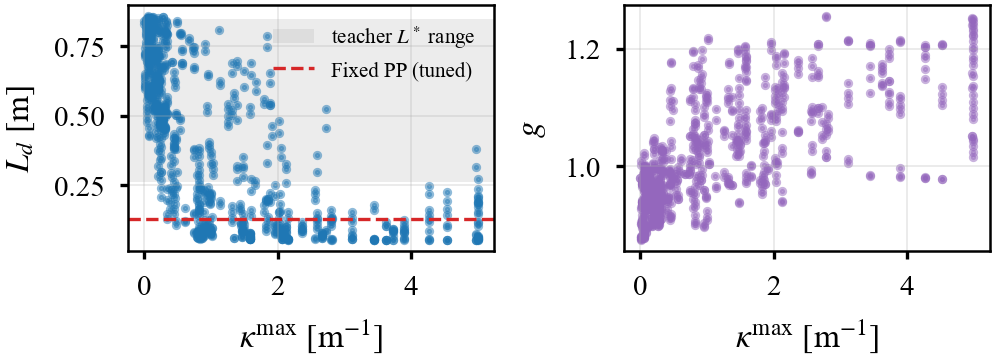
\includegraphics[width=\columnwidth]{fig7_interp.png}
\vskip -0.5pc
\caption{Lookahead and gain chosen by the joint RL--PP agent (seed 0) while driving the unseen Montreal circuit: $L_d$ and $g$ versus previewed curvature. Shaded: teacher's $L^{*}$ range; dashed: tuned Fixed PP.}\label{fig:interp}
\vskip -1pc
\end{figure}

\subsection{Statistical evidence}
\begin{table*}[t]
\caption{Pairwise RMSE differences A$-$B in cm across all eight test circuits (negative favours A; 95\% bootstrap interval over circuits and training seeds; exact Wilcoxon test). Left: against the extracted references. Right: the same comparison against the true F1TENTH centerlines, recomputed from the stored trajectories.}\label{tab:comp}
\centering
\resizebox{\textwidth}{!}{%
\setlength{\tabcolsep}{2pt}
\renewcommand{\arraystretch}{0.88}%
\begin{tabular}{lccccc|cc}
\toprule
 & \multicolumn{5}{c|}{Extracted reference} & \multicolumn{2}{c}{True centerline}\\
A vs B & Diff. & 95\% CI & Better & $p$ & Holm & Diff. & 95\% CI\\
\midrule
\tabinput tables/tab_comparisons.tex
\bottomrule
\end{tabular}}
\end{table*}
In all four primary comparisons (Table~\ref{tab:comp}) the same controller is better on all eight circuits, so $p=0.0078$, which remains below 0.05 after Holm correction ($p=0.031$). With eight circuits this only says that all circuits agree; effect sizes are given by the intervals, which describe variation over these circuits and seeds, not over other simulators, scales or vehicles.

\subsection{Threats to validity}
\begin{itemize}\setlength{\itemsep}{1pt}\setlength{\parskip}{0pt}\setlength{\topsep}{2pt}
\item \textbf{Extraction error and spacing.} Differences below about 1~cm are within the extraction error (Table~\ref{tab:truecl}). The Austin test reference does not close exactly (Table~\ref{tab:spacing}); closing it changes RMSE by at most 0.012~cm and no lap outcome. Waypoints are \VspMin--\VspMax~cm apart, which may disadvantage the expert, whose target is the next waypoint, whereas PP interpolates its lookahead point.
\item \textbf{PPO budget and settings.} $2$--$3\times10^6$ steps per run; of the fine-tuning settings only the behaviour-cloning weight was varied ($\lambda\in\{0.1,1,10\}$, three seeds), while initial noise, learning rate and critic warm-up were fixed. Our results show that PPO did not improve the policy under these settings, not that it cannot.
\item \textbf{RL--PP adaptation.} Scale, ranges, teacher, reward weights and budget differ from~\cite{elgouhary2026} (Table~\ref{tab:adapt}); results characterize our adaptation.
\item \textbf{Plants and scale.} Bead-PP controls for the plant for one law and one speed; the main comparison uses a kinematic car (dynamic model: Table~\ref{tab:dynamic}); tracks are shrunk \VscaleLo--\VscaleHi$\times$.
\item \textbf{Exposure and scope.} Three test circuits were known when the reward was designed, and a preliminary run touched the test circuits (Section~4.1); five seeds; only 50 of the 150 test contours in each synthetic set; simulation only. Not yet tested: sensor noise and true-scale circuits with real steering limits.
\end{itemize}

\section{Conclusion}
Under shared paths, measures and lap rule, we compared learning that replaces a geometric tracking law with learning integrated into it, on held-out circuits. The DAgger-trained bead matched its hand-written teacher; taught by the PP law, it came within \VcmpBppTeachDiff~cm of that law on the extracted references and matched it, and tuned PP on the car, against the true centerlines, so the teacher, more than the network, limited imitation. With our PPO budget and settings, PPO did not improve the imitation policy, whether started from scratch or fine-tuned, with either reward or any behaviour-cloning weight tried. A tuned PP law was more accurate than every learned controller that did not imitate it, on the car and on the bead, so the gap comes from the control law rather than the vehicle; it shrinks to \VtruePoneDiff~cm against the true centerlines but keeps its sign on every circuit. Our RL-tuned PP reproduced the qualitative schedule of~\cite{elgouhary2026} but followed a teacher with long lookaheads. A naive protocol would have reversed these conclusions. A well-tuned PP law is thus a strong baseline (tuned Stanley, which regulates the front axle, less so). On a dynamic car it stays the most accurate car controller only after re-tuning, with a smaller margin, so baselines should be tuned on the vehicle model used for comparison. Integrating learning with PP, for example as a learned residual, is a more promising direction than replacing it, together with hardware tests.

\section*{Declarations}
\subsection*{Conflict of Interest}
The authors have no financial or personal interests to declare that are relevant to this work.

\subsection*{Authors' Contributions}
[To be completed by the authors: the contributions of Dileep Banothu and N. Sanjay Varma.]

\subsection*{Funding}
Not applicable.

\subsection*{Data Availability}
The code, data split, trained checkpoints, raw test trajectories and the scripts that generate every table and number of this paper can be obtained from the corresponding author upon request. The F1TENTH centerlines come from the public F1TENTH racetrack collection.

\begin{reference}
\bibitem{okelly2020} M. O'Kelly, H. Zheng, D. Karthik, and R. Mangharam, ``F1TENTH: An open-source evaluation environment for continuous control and reinforcement learning,'' \textit{Proc. of the NeurIPS 2019 Competition and Demonstration Track}, PMLR, vol. 123, pp. 77-89, 2020.
\bibitem{coulter1992} R. C. Coulter, ``Implementation of the pure pursuit path tracking algorithm,'' Technical Report CMU-RI-TR-92-01, Robotics Institute, Carnegie Mellon University, 1992.
\bibitem{snider2009} J. M. Snider, ``Automatic steering methods for autonomous automobile path tracking,'' Technical Report CMU-RI-TR-09-08, Robotics Institute, Carnegie Mellon University, 2009.
\bibitem{elgouhary2026} M. Elgouhary and A. S. El-Wakeel, ``Learning to tune pure pursuit in autonomous racing: Joint lookahead and steering-gain control with PPO,'' \textit{arXiv preprint} arXiv:2602.18386, 2026.
\bibitem{schulman2017} J. Schulman, F. Wolski, P. Dhariwal, A. Radford, and O. Klimov, ``Proximal policy optimization algorithms,'' \textit{arXiv preprint} arXiv:1707.06347, 2017.
\bibitem{ross2011} S. Ross, G. J. Gordon, and J. A. Bagnell, ``A reduction of imitation learning and structured prediction to no-regret online learning,'' \textit{Proc. of the 14th International Conference on Artificial Intelligence and Statistics (AISTATS)}, pp. 627-635, 2011.
\bibitem{hoffmann2007} G. M. Hoffmann, C. J. Tomlin, M. Montemerlo, and S. Thrun, ``Autonomous automobile trajectory tracking for off-road driving: Controller design, experimental validation and racing,'' \textit{Proc. of the American Control Conference}, pp. 2296-2301, 2007.
\bibitem{rajamani2012} R. Rajamani, \textit{Vehicle Dynamics and Control}, 2nd ed., Springer, New York, 2012.
\bibitem{kong2015} J. Kong, M. Pfeiffer, G. Schildbach, and F. Borrelli, ``Kinematic and dynamic vehicle models for autonomous driving control design,'' \textit{Proc. of the IEEE Intelligent Vehicles Symposium}, pp. 1094-1099, 2015.
\bibitem{heilmeier2020} A. Heilmeier, A. Wischnewski, L. Hermansdorfer, J. Betz, M. Lienkamp, and B. Lohmann, ``Minimum curvature trajectory planning and control for an autonomous race car,'' \textit{Vehicle System Dynamics}, vol. 58, no. 10, pp. 1497-1527, 2020.
\bibitem{betz2022} J. Betz, H. Zheng, A. Liniger, U. Rosolia, P. Karle, M. Behl, V. Krovi, and R. Mangharam, ``Autonomous vehicles on the edge: A survey on autonomous vehicle racing,'' \textit{IEEE Open Journal of Intelligent Transportation Systems}, vol. 3, pp. 458-488, 2022.
\bibitem{kiran2022} B. R. Kiran, I. Sobh, V. Talpaert, P. Mannion, A. A. Al Sallab, S. Yogamani, and P. P\'erez, ``Deep reinforcement learning for autonomous driving: A survey,'' \textit{IEEE Transactions on Intelligent Transportation Systems}, vol. 23, no. 6, pp. 4909-4926, 2022.
\bibitem{kober2013} J. Kober, J. A. Bagnell, and J. Peters, ``Reinforcement learning in robotics: A survey,'' \textit{International Journal of Robotics Research}, vol. 32, no. 11, pp. 1238-1274, 2013.
\bibitem{schulman2016} J. Schulman, P. Moritz, S. Levine, M. Jordan, and P. Abbeel, ``High-dimensional continuous control using generalized advantage estimation,'' \textit{Proc. of the International Conference on Learning Representations (ICLR)}, 2016.
\bibitem{andrychowicz2021} M. Andrychowicz, A. Raichuk, P. Sta\'nczyk, M. Orsini, S. Girgin, R. Marinier, L. Hussenot, M. Geist, O. Pietquin, M. Michalski, S. Gelly, and O. Bachem, ``What matters in on-policy reinforcement learning? A large-scale empirical study,'' \textit{Proc. of the International Conference on Learning Representations (ICLR)}, 2021.
\bibitem{haarnoja2018} T. Haarnoja, A. Zhou, P. Abbeel, and S. Levine, ``Soft actor-critic: Off-policy maximum entropy deep reinforcement learning with a stochastic actor,'' \textit{Proc. of the 35th International Conference on Machine Learning (ICML)}, pp. 1861-1870, 2018.
\bibitem{evans2023} B. D. Evans, H. W. Jordaan, and H. A. Engelbrecht, ``Comparing deep reinforcement learning architectures for autonomous racing,'' \textit{Machine Learning with Applications}, vol. 14, 100496, 2023.
\bibitem{pomerleau1989} D. A. Pomerleau, ``ALVINN: An autonomous land vehicle in a neural network,'' \textit{Advances in Neural Information Processing Systems 1}, pp. 305-313, 1989.
\bibitem{otsu1979} N. Otsu, ``A threshold selection method from gray-level histograms,'' \textit{IEEE Transactions on Systems, Man, and Cybernetics}, vol. 9, no. 1, pp. 62-66, 1979.
\bibitem{zhang1984} T. Y. Zhang and C. Y. Suen, ``A fast parallel algorithm for thinning digital patterns,'' \textit{Communications of the ACM}, vol. 27, no. 3, pp. 236-239, 1984.
\bibitem{raffin2021} A. Raffin, A. Hill, A. Gleave, A. Kanervisto, M. Ernestus, and N. Dormann, ``Stable-Baselines3: Reliable reinforcement learning implementations,'' \textit{Journal of Machine Learning Research}, vol. 22, no. 268, pp. 1-8, 2021.
\end{reference}

\end{document}
